\begin{frame}{ToF}
    \begin{itemize}
        \item ToF = Time of Flight
        \item It is the time it takes for a signal to travel from the sender to the receiver
    \end{itemize}
\end{frame}

\begin{frame}{ToF: Distance measurement}
    \begin{columns}
        \column{0.4\textwidth}
        \begin{itemize}
            \item Role models: bat, dolphin
        \end{itemize}

        \begin{figure}
            \animategraphics[width=0.8\textwidth]{10}{animations/fledermaus-}{0}{14}
            \caption{\cite{wikipedia2023laufzeitmessung}}
        \end{figure}

        \column{0.6\textwidth}
        \onslide<2->
        {
            \begin{itemize}
                \item Technical: Ultra sonic, radar, laser
            \end{itemize}

            \begin{figure}
                \includesvg[width=0.8\textwidth]{graphics/distance-measurement.svg}
                \caption{\cite{wikipedia2023laufzeitmessung}}
            \end{figure}
        }
    \end{columns}

    \onslide<3->{
        \begin{equation*}
            d = \frac{c \cdot ToF}{2}
        \end{equation*}
    }
\end{frame}

\begin{frame}{ToF: Flow measurement}
    \begin{itemize}
        \item For fluids ToF can also be used to measure the flow rate (flow speed)
              \begin{itemize}
                  \item E.g., sonico NANO, sonico EDGE
              \end{itemize}
    \end{itemize}

    \begin{figure}
        \includegraphics[width=0.7\textwidth]{diagrams/flow-tof.pdf}
    \end{figure}
\end{frame}

\begin{frame}{ADC}
    \begin{itemize}
        \item ADC = Analog to Digital Converter
    \end{itemize}

    \onslide<2->{
        \begin{figure}
            \includegraphics[width=\textwidth]{diagrams/sensor-adc.pdf}
        \end{figure}
    }
\end{frame}

\begin{frame}{TDC}
    \begin{itemize}
        \item TDC = Time to Digital Converter
        \item Similar to ADC, but to directly measure the time (like a stopwatch)
    \end{itemize}

    \begin{columns}
        \column{0.45\textwidth}
        \begin{figure}
            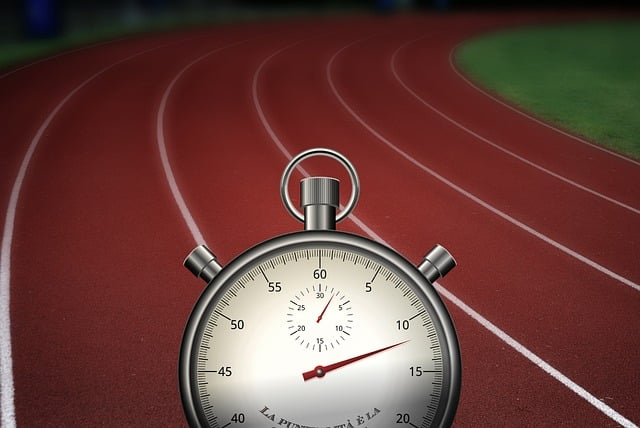
\includegraphics[width=\textwidth]{graphics/stopwatch.jpg}
        \end{figure}

        \column{0.55\textwidth}
        \onslide<2->{
            \begin{figure}
                \includegraphics[width=\textwidth]{diagrams/tdc.pdf}
            \end{figure}
        }
    \end{columns}

\end{frame}
